\chapter{High fidelity prototype}


\section{Prototype}
The last iteration of the prototype is the High fidelity prototype. This prototype is as close as it gets to the final product. Therefore the focus of this iteration was to make the prototype look and feel as nice as possible.\\
This prototype is made in a real programming language and in the style which matches the windows store app's.\\
These app's are commonly very simple and very easy to use. This helps achieving our most important usability and user experience goals.\\
Since the app is simple it doesn't over complicate the task at hand by fancy graphics. This makes the app helpful for the caregivers and hopefully also satisfying to use too. With this in mind it achieves most usability goals - effectiveness, efficiency, learnable and memorable. These goals are all achieved when the app is simple and manageable.\\
As it shows with the comparison below, the prototype is simpler and more beautiful than the mid fidelity prototype.\\
\begin{figure}[H]
\centering
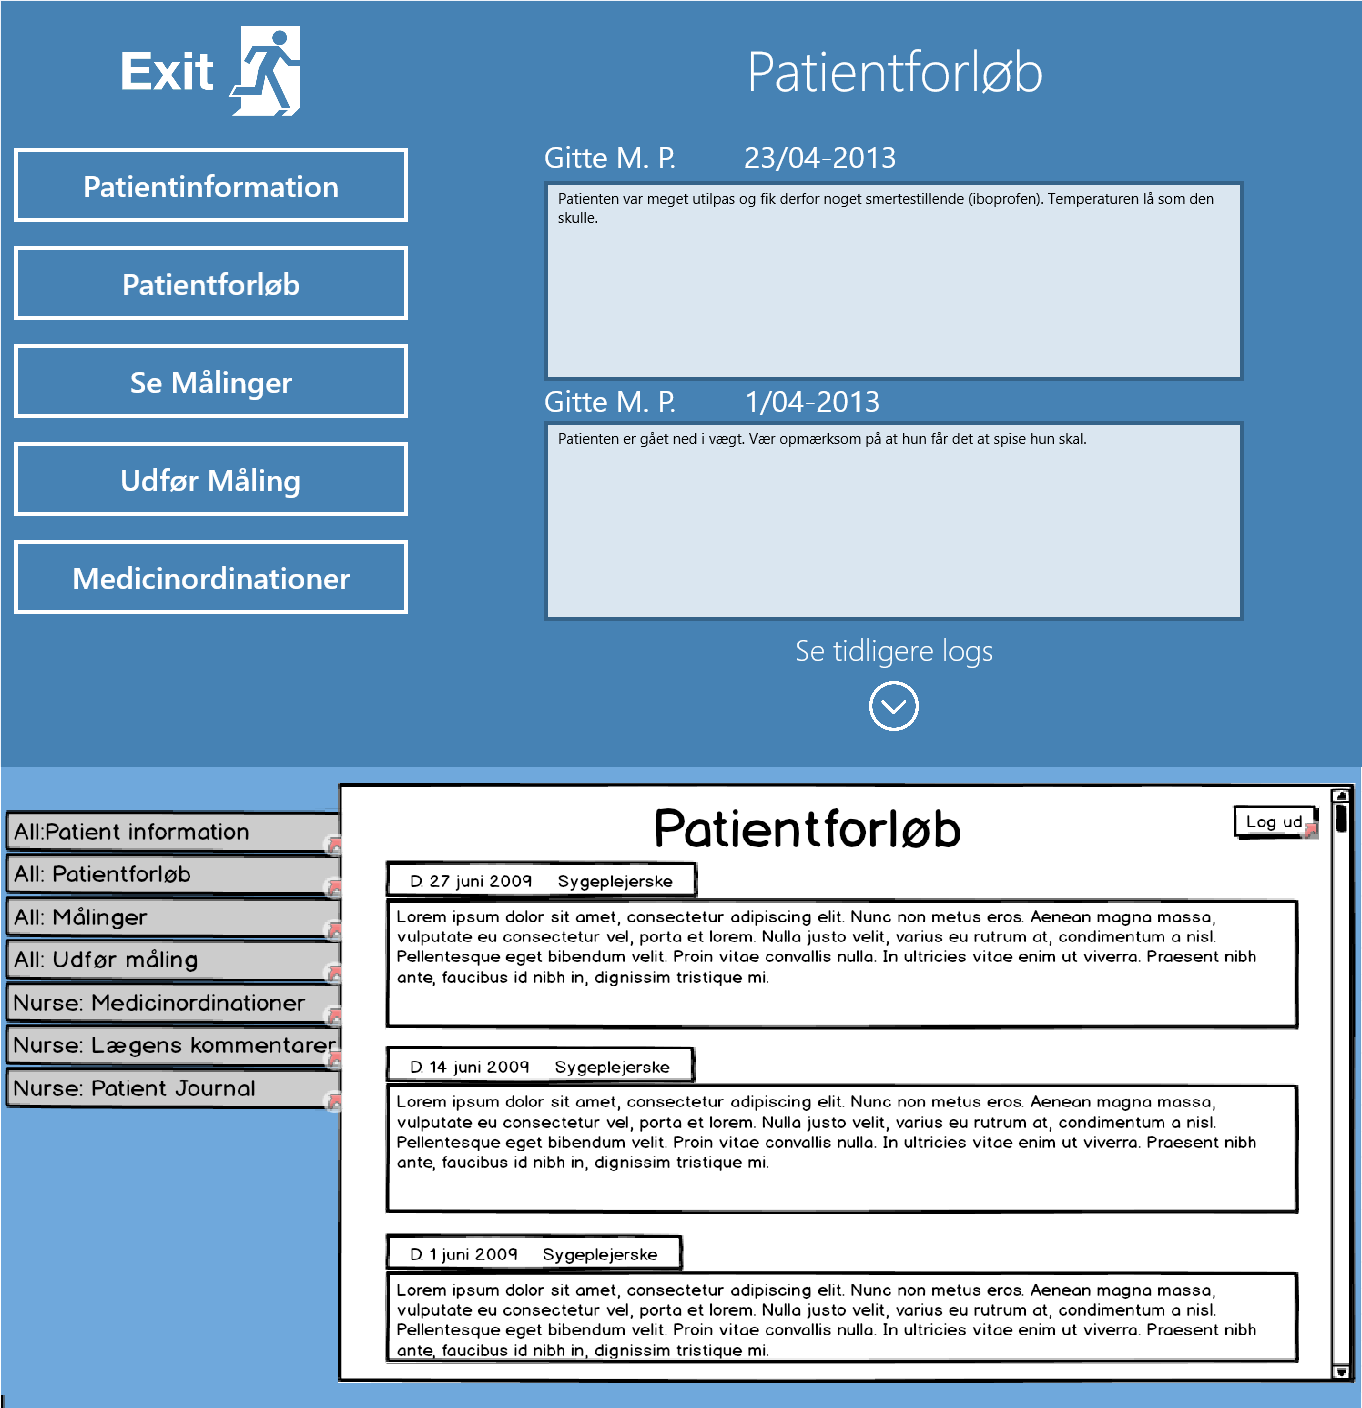
\includegraphics[width=.7\textwidth]{billeder/midhigh_compare.png}
\end{figure}

\section{Obtaining usability goals}
hest

\section{Obtaining user experience goals}
Hest

\section{Peer review}
Hest

\subsection{Results of hi-fi peer review}
Hest